\documentclass[12pt]{article}
\usepackage[a3paper,landscape]{geometry}

\usepackage[poster]{tcolorbox}
\usepackage{pagecolor}
\usepackage{background}
\usepackage{mdframed}
\pagestyle{empty}
\pagecolor{red}

\begin{document}
% \begin{tcbposter}[
% coverage = {spread,
% interior style={top color=cyan,bottom color=cyan!50!red}
% },

% poster = {columns=3,rows=2},

% boxes = {fonttitle = \bfseries\Large\scshape},
% fontsize = 16pt
% ]

% \posterbox{name=title,column=2,span=2,above=bottom}{
    
%     \underline{David Amaro-Alcala}, Barry C. Sanders, Hubert de Guise
% }
% \posterbox[adjusted title = Summary, colframe = teal!50!black, colback=teal!50]{
    
%     column = 1,
%     name=project, 
%     between=top and bottom
% }{
% {\Huge We characterise a set of generators of universal qutrit gates, via the \textbf{average gate fidelity}.}
% }

% \posterbox[adjusted title = Characterise]{
%     name=result, 
%     column = 2,row =1
% }{
% {
% Randomised Benchmarking is a method used to assess the quality of quantum gates
% by estimating the average fidelity of a randomly selected set of gates from a
% particular set. The fidelity is determined by comparing the behaviour of the
% gates to the expected behaviour of ideal gates that would make up the identity
% operation.
% }
% 
\includegraphics[width=\textwidth]{auxiliary figures/crazy-scientist.pdf}
% }



% \posterbox[adjusted title = T gate]{
%     name=result1, 
%     column = 3,row =1
% }{
% Randomised Benchmarking (RB) is commonly used to characterise Clifford gates,
% but in order for a quantum computer to surpass a classical computer, it must
% also be able to implement a T gate in addition to the Clifford gate set. T gates
% are not part of the Clifford group, so an extension of RB is required to
% characterize T gates.
% \begin{center}
% 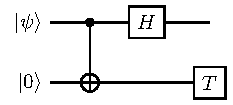
\includegraphics[width=0.5\textwidth]{auxiliary figures/universal-circuit.pdf}
% \end{center}
% A \textbf{qutrit} is a three-level system; that is, a system with two excited states.
% Qutrits offer advantages with respect to qubits.
% Moreover, qutrits nowadays are widely implemented, for example, in ion traps.
% }

% \posterbox[adjusted title = The HDG]{
    
%     name=result2, 

% column = 2,
% between = result1 and title,
    

    
% }{




% Common Randomised Benchmarking schemes assume that the gates, being
% characterised, correspond to the physical implementation of a group.
% We were interested in the minimal (in order) group that included the T
% gate. Such group, which we call HyperDihedral, is generated by the following three matrices:

% \begin{center}
% 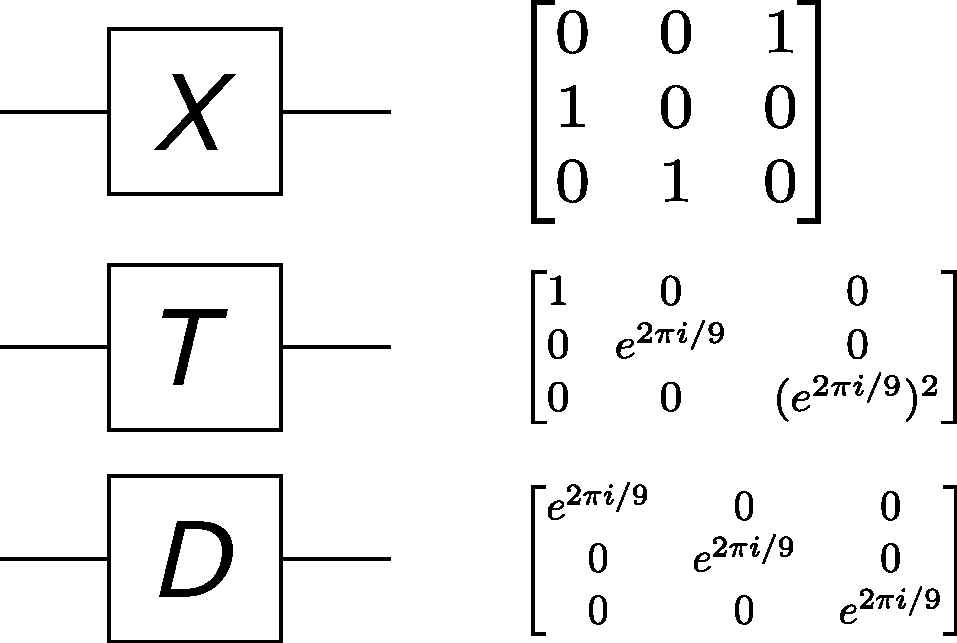
\includegraphics[width=0.7\textwidth]{auxiliary figures/matrices.pdf}
% \end{center}
% }

% \posterbox[adjusted title = Results]{
    
%     name=conclusion1, 
%     column = 3,

% between = result and title,
% % between = result1 and title,
    

    
    
    
    
% }{
% We obtained an expression for the average gate fidelity over a HDG
% implementation. Our formalism is valid under state preparation and
% measurement imperfections and for gate-dependent errors. These two
% conditions make our method part of the state-of-the-art in Randomised
% Benchmarking schemes.


% \begin{center}
% \includegraphics[width=0.8\textwidth]{auxiliary figures/spplotandagf.pdf}
% \end{center}
% }



\begin{tcbposter}[
coverage = {spread, interior style={top color=cyan,bottom color=cyan!50!red} },
poster = {columns=3,rows=2},
boxes = {fonttitle = \bfseries\Large\scshape},
fontsize = 16pt
]
\posterbox[adjusted title = Summary, colframe = teal!50!black, colback=teal!50]{
    column = 1,
    name=project, 
    between=top and bottom
}{
{\Huge We characterise a set of generators of universal qutrit gates, via the \textbf{average gate fidelity}.}
}

\posterbox[adjusted title = Background]{
    name=result, 
    column = 2,row =1,span = 2
}{
\begin{minipage}{0.49\linewidth}
Randomised Benchmarking is a method used to assess the quality of quantum gates
by estimating the average fidelity of a randomly chosen set of gates from a
particular set. The fidelity is determined by comparing the behaviour of the
gates to the expected behaviour of ideal gates that would make up the identity
operation.

\includegraphics[width=\textwidth]{auxiliary figures/crazy-scientist.pdf}
\end{minipage}
\hspace{0.02\textwidth}
\begin{minipage}{0.45\linewidth}
Randomised Benchmarking (RB) is commonly used to characterise Clifford gates,
but in order for a quantum computer to surpass a classical computer, it must
also be able to implement a T gate in addition to the Clifford gate set. T gates
are not part of the Clifford group, so an extension of RB is required to
characterize T gates.
\begin{center}
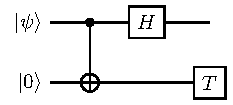
\includegraphics[width=0.45\textwidth]{auxiliary figures/universal-circuit.pdf}
\end{center}
A \textbf{qutrit} is a three-level system; that is, a system with two excited states.
Qutrits offer advantages with respect to qubits.
Moreover, qutrits nowadays are widely implemented, for example, in ion traps.
\end{minipage}
}


% inferior block
\posterbox[adjusted title = Results]{
    name=result, 
    column = 2,row =2,span = 2
}{
\begin{minipage}{0.45\linewidth}
Common Randomised Benchmarking schemes assume that the gates, being
characterised, correspond to the physical implementation of a group.
We were interested in the minimal (in order) group that included the T
gate. Such group, which we call HyperDihedral, is generated by the following three matrices:
\end{minipage}
\hspace{0.02\textwidth}
\begin{minipage}{0.45\linewidth}
We obtained an expression for the average gate fidelity over a HDG
implementation. Our formalism is valid under state preparation and
measurement imperfections and for gate-dependent errors. These two
conditions make our method part of the state-of-the-art in Randomised
Benchmarking schemes.
\begin{center}
\includegraphics[width=0.8\textwidth]{auxiliary figures/spplotandagf.pdf}
\end{center}
\end{minipage}
}
\end{tcbposter}
\end{document}